\subsection{The cell and the cellular membrane}
\label{sec:cell}
Cells are the fundamental units of every living being, which can be made up of one cell (unicellular) or more (multicellular).
Indipendently on how big and complex an organism could be, each cell always maintains its individuality and its independence, but maintaining common structural proprieties.

The internal volume is defined by the \textit{cytoplasm}, which is a liquid solution where several insoluble particles stands, such as enzimes, \textit{RNA} and metabolites.
Moreover, it is possible to distinguish multiple organelles, such as \textit{ribosomes}, the \textit{endoplasmic reticulum}, the \textit{golgi comples},\textit{lisosomes} and the \textit{nucleus} (figure \ref{fig:cell}).
In particular, this last one has a the role of contain the genome, represented by the \textit{DNA}.

\begin{figure}[H]
\centering
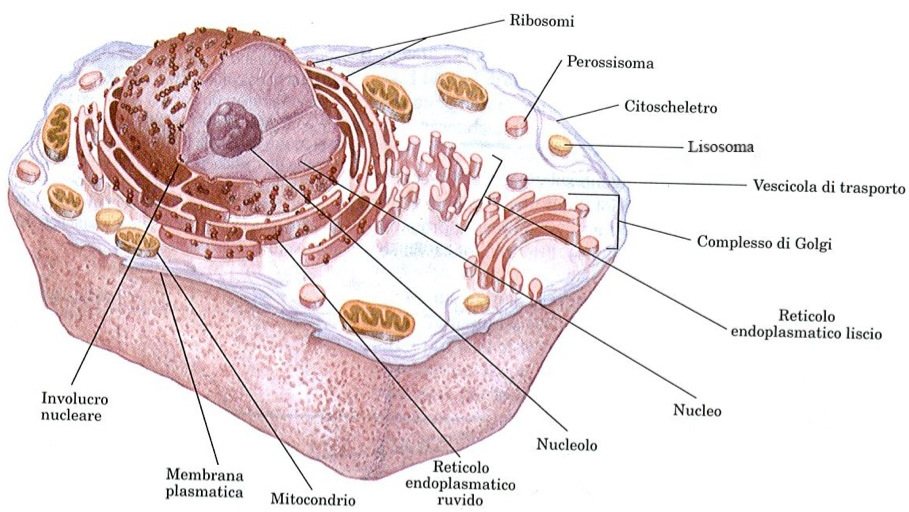
\includegraphics[width=\textwidth, keepaspectratio]{img/intro/cell.png}
\caption[The Cell]{Schematic representation of a cell.}
\label{fig:cell}
\end{figure}

\subsection{The DNA}
\label{sec:genica}
The \textit{DNA} was been isolated for the first time by the German doctor Friederick Miescher in 1869, while in the same decade the English biologist Charles Darwin was publishing \textit{On the Origin of the Species} and the  Augustinian friar scientist was communicating his results on the pees to the Brunn Natural History Society.

Because the substance isolated by Miescher was white, lightly acid and present only into the cells nuclei, it was been termed \textit{Nucleic Acid}.
Name modified afterwards in \gls{dna}, to distinguish is from the another one, very similar, the \gls{rna}.

These two molecules are constituted by \textit{nucleotides}, constituted by a nitrogen base, deoxyribose sugar and a phosphate group.
We distinguish two nitrogen bases, purines and pyrimidines.
Inside the \gls{dna}, we have two \textit{pyrimidines}, \textit{adenine (A)} and \textit{guanine (G)}, and two \textit{pyrimidines}, the \textit{Cytosine (C)} and the \textit{Thimine (T)}  .
Inside \gls{rna} \textit{Thymine} is substituted by the \textit{Uracil (U)}.

\begin{figure}[H]
\centering
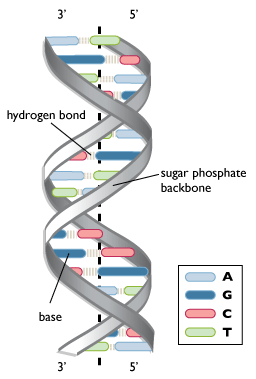
\includegraphics[width=\textwidth, keepaspectratio]{img/intro/dna1.png}
\caption[the \gls{dna}]{Schematic representation of double-stranded filament structure of \gls{dna}. The legend report the four nitrogen bases, Adenine, Guanine, Cytosine and Thymine.}
\label{fig:dna}
\end{figure}

\gls{dna} structure (figure \ref{fig:dna}) was discovered, in the 50's, by the American scientist James Watson, the French physicist Francis Crick and the English chemist-physicist Rosalind Franklyn.
According to their model the \gls{dna} is a double-stranded filament, where Adenines can pair only with Thymines and Guanines only with Cytosines.
The four bases constitute the alphabet for the genetic message.

\gls{dna} is folded on itself (\textit{\gls{dna} packaging}, thanks to specific "beads" called \textit{nucleosomes}, which themselves consist of eight proteins with tails, called \textit{histones}, that have the \gls{dna} wrapped on them.
This mechanism enables to store around 2 meters of chromatin inside a nucleus of a 2-10 micron diameter, when referring to Human specie.

Moreover, the \gls{dna} contains the \textit{genes}, particular sections containing relevant information for building proteins and other fundamental molecules for the cellular behavior regulation.
Each gene is localized on a precise position of a \textit{Chromosome}, which are in different number for each specie.
Each chromosome is constituted by \gls{dna} within thousands genes.

\begin{figure}[H]
\centering
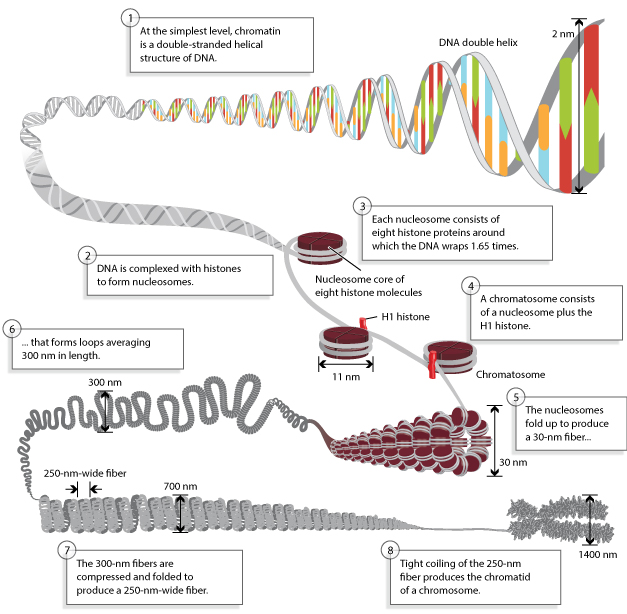
\includegraphics[width=\textwidth, keepaspectratio]{img/intro/dna2.jpg}
\caption[Chromosomes and \gls{dna}]{Representation of the relation between \gls{dna} and Chromosomes.
Inside the cell nucleus there are pairs of chromosome, constituted by chromatin, which fundamental unit is constituted by nucleosomes, on which the \gls{dna} is wrapped around, containing the genetic information in gene form. (image adapted from \cite{Annunziato2008})}
\label{fig:dnachromosome}
\end{figure}

Figure \ref{fig:dnachromosome} better helps  to understand the relationship between chromosomes, chromatin, nucleosomes and genes.

It is important to underlying that since some decades ago the Central Dogma of Molecular Biology was founded on the transcription - translation principle, where \gls{dna} was transcribed in \gls{rna}, which subsequently it would have been translated into protein.

Nowadays, we know that the gene transcription is regulated by several mechanisms, and moreover, the translation is not the only process fated for \gls{rna}.

Indeed, for a transcription of a gene, there are some requisites to be respected, such as the accessible of that specific part of the chromatin, or the binding of specific proteins enabling the accession to the gene region, or the phosphorylation process, which modifies the state of specific histones.
  

%La figura \ref{Fig:dnachromosome} a pagina \pageref{Fig:dnachromosome} aiuta meglio a comprendere la relazione che intercorre tra DNA, gene e cromosoma. 
%Gli introni sono regioni non codificanti spesso presenti nei geni eucarioti, eliminate attraverso lo \textit{splicing}: solo gli esoni codificano per le proteine. 
%\'E importante sottolineare che finora gli introni erano considerati ''DNA spazzatura'', senza alcuna particolare funzione, ma oggi i ricercatori hanno scoperto che ricoprono un ruolo importante. 
%Il dato sorprendente è che esistono sequenze di introni estremamente conservate tra le diverse specie che hanno una funzione nella corretta formazione degli RNA messaggeri. Non è infatti tanto il numero di geni quanto il modo in cui il loro funzionamento è regolato a rendere l'uomo, uomo e il topo, topo. Basti pensare che l'uomo ha circa lo stesso numero di geni del topo.
%
%\section{L'espressione genica}
%\label{sec:genica}
%La chiave per comprendere i complessi meccanismi della regolazione del metabolismo cellulare consiste nell'interpretare il flusso di informazioni che hanno luogo secondo regole comuni alla maggior parte degli organismi viventi. Le informazioni sono conservate all'interno della molecola del DNA e possono essere sia riprodotte per duplicazione che utilizzate per produrre un vero e proprio messaggio, che ha come obiettivo finale una ben determinata azione chimica. 
%L'unità fondamentale dell'ereditarietà, il gene, è un frammento di DNA in grado di codificare un prodotto specifico o, in generale, una o più funzioni correlate. 
%Il processo di espressione genica per assemblare la struttura amminoacidica di una proteina avviene in due fasi:
%\begin{itemize}
%\item \textbf{trascrizione:} un enzima (\textit{RNA polimerasi}) catalizza la sintesi di una molecola di RNA messaggero (mRNA) usando il gene come modello.
%\item \textbf{traduzione:} le informazioni contenute nella sequenza dell'\textit{mRNA} determinano la sintesi di uno specifico polipeptide, eseguita dal ribosoma.
%\end{itemize}
%
%Volendo apprezzare con maggiore dettaglio il processo di espressione genica, va anzitutto ricordato che la fase di trascrizione ha inizio quando l'enzima RNA polimerasi si lega ad una regione del DNA chiamata \textbf{promotore}. 
%Un promotore, tipicamente localizzato in prossimità dei geni, è una regione del DNA in cui le proteine come i fattori di trascrizione possono legare. 
%Questi siti contribuiscono all'attivazione della trascrizione delle successive sequenze di geni aumentandone oppure inibendone la trascrizione. 
%In prossimità del complesso formato da RNA polimerasi e DNA \textit{promoter}, la doppia elica del DNA si srotola parzialmente e l'enzima può muoversi lungo il filamento modello nella direzione 3'-5'\footnote{3'-5' indica la direzionalità da un estremo all'altro di un singolo filamento di acido nucleico. Il verso opposto, tipicamente del filamento complementare, viene indicato con 5'-3'.}, polimerizzando nella direzione opposta.
%Dal momento che il promotore impone alla polimerasi l'orientamento sul DNA e che la polimerizzazione può avvenire in una sola direzione (5'-3'), la polimerasi è obbligata a scegliere come modello uno solo dei due filamenti complementari. 
%\'E da notare che non sempre viene selezionato lo stesso filamento di DNA, e non sempre nello stesso punto. Ciò dipende dalla posizione del gene che la polimerasi deve trascrivere.
%%Se da un lato deve essere scelto un unico filamento di DNA, dall'altro non è detto che la scelta ricada sempre sullo stesso: ciò dipende dal gene. 
%La parte del gene che viene trascritta è detta \textbf{trascritto}, ed è una copia di DNA che dà vita ad una molecola di \textbf{RNA messaggero (mRNA)}.
%
%La sintesi della molecola di mRNA ha termine quando l'enzima RNA polimerasi incontra una sequenza particolare nel filamento di DNA modello che segnala la fine del processo.
%
%L'espressione genica è dunque caratterizzata da un flusso di informazioni che va dal DNA all'RNA, alle proteine. 
%Mentre DNA e RNA sono scritti con un alfabeto in base 4, nel caso delle proteine l'alfabeto è in base 20.
%Il termine traduzione indica infatti il passaggio da un alfabeto a 4 lettere (le basi azotate degli acidi nucleici) a un alfabeto a 20 lettere (tanti quanti sono gli amminoacidi costitutivi delle proteine presenti in natura).